\documentclass[a4paper, 7pt, landscape]{scrartcl}
\usepackage[german]{babel}
\usepackage[utf8]{inputenc}
\usepackage{multicol}
\usepackage{geometry}
\usepackage{graphicx}
\usepackage{wrapfig}
\usepackage{enumitem}
\usepackage{fancyhdr}
\usepackage{index}
\usepackage{sectsty}
\usepackage{mwe}
\usepackage{comment}
\usepackage{lipsum}
\usepackage{titlesec}
\usepackage[dvipsnames]{xcolor}
\usepackage{amsmath}
\usepackage{amssymb}


%Define Math Commands:
\newcommand*{\field}[1]{\mathbb{#1}}%
\newcommand{\Mod}[1]{\ (\mathrm{mod}\ #1)}

%Image Folder:
\graphicspath{{../img/}}

%format
\geometry{top=0.4cm,left=0.5cm,right=0.5cm,bottom=0.4cm}
\setlist{topsep=0pt, leftmargin=5mm, nolistsep}

% Code Snippets
\usepackage{courier} %% Sets font for listing as Courier.
\usepackage{listings}

\definecolor{javared}{rgb}{0.6,0,0} % for strings
\definecolor{sectionColor}{HTML}{7cbad4}
\definecolor{subSectionColor}{HTML}{c7e5b6}
\definecolor{subSubSectionColor}{HTML}{ffeca9}
\definecolor{royalBlue}{HTML}{4A1FBF}
\definecolor{midnightBlue}{HTML}{191970}
\definecolor{codeBackground}{RGB}{245,245,245}
\definecolor{gray}{rgb}{0.5,0.5,0.5}
\definecolor{lightgray}{rgb}{.9,.9,.9}
\definecolor{darkGreen}{RGB}{0,150,0}
\definecolor{DarkPurple}{rgb}{0.4, 0.1, 0.4}

%define Javascript language
\lstdefinelanguage{JavaScript}{
keywords={typeof, new, true, false, catch, function, return, null, catch, switch, var, if, in, while, do, else, case, break, const, let, var, console, log},
keywordstyle=\color{blue}\bfseries,
ndkeywords={class, export, boolean, throw, implements, import, this},
ndkeywordstyle=\color{darkgray}\bfseries,
identifierstyle=\color{black},
sensitive=false,
comment=[l]{//},
morecomment=[s]{/*}{*/},
commentstyle=\color{purple}\ttfamily,
stringstyle=\color{red}\ttfamily,
morestring=[b]',
morestring=[b]"
}

\lstset{
frame=none,
captionpos=b,
escapeinside={*'}{'*},
language=haskell,
tabsize=2,
commentstyle=\it,
stringstyle=\mdseries\rmfamily,
showspaces=false,
keywordstyle=\bfseries\color{RoyalBlue},
backgroundcolor=\color{lightgray},
columns=flexible,
basicstyle=\small\sffamily,
showstringspaces=false,
morecomment=[l]\%,
aboveskip = 0.2em,
belowskip = 0.2em
}




% Define Section Format
\titleformat{name=\section}[block]{\sffamily\small}{}{0pt}{\colorsection}
\titlespacing*{\section}{0pt}{0pt}{0pt}
\newcommand{\colorsection}[1]{%
\colorbox{sectionColor!80}{\parbox{0.98\linewidth}{\vspace{-1pt}\color{black}\ #1 \vspace{-2pt}}}}

% Define Subsection Format
\titleformat{name=\subsection}[block]{\sffamily\small}{}{0pt}{\colorsubsection}
\titlespacing*{\subsection}{0pt}{0pt}{0pt}
\newcommand{\colorsubsection}[1]{%
\colorbox{subSectionColor!80}{\parbox{0.98\linewidth}{\vspace{-1pt}\color{black}\ #1 \vspace{-2pt}}}}

% Define SubSubsection Format
\titleformat{name=\subsubsection}[block]{\sffamily\small}{}{0pt}{\colorsubsubsection}
\titlespacing*{\subsubsection}{0pt}{0pt}{0pt}
\newcommand{\colorsubsubsection}[1]{%
\colorbox{subSubSectionColor!60}{\parbox{0.98\linewidth}{\vspace{-1pt}\color{black}\ #1 \vspace{-2pt}}}}


% -----------------------------------------------------------------------
\begin{document}
    %	\pagecolor{p}
    %	\color{t}
    \setlength{\columnseprule}{0.4pt}
    \footnotesize
    \begin{multicols*}{3}

        %! Author = Philipp Emmenegger
%! Date = 10/06/2021

\section{Introduction}
\textbf{Formal Methods}
\begin{itemize}
    \item Application of theoretical computer science fundamentals
    \item Logic calculi
    \item Formal languages
    \item Automata theory
    \item Program semantics
    \item Type systems
    \item Algebraic data types
\end{itemize}

\textbf{Formal Language}
\begin{itemize}
    \item Set of strings of symbols
    \item Constrained by specific rules
    \item Programming languages
    \item Usage: Specify, invent, transform, analyse, verify, reason about programming languages
    \item Informal: living natural languages
\end{itemize}

\subsection{Execution-based vs. Rule-based thinking}
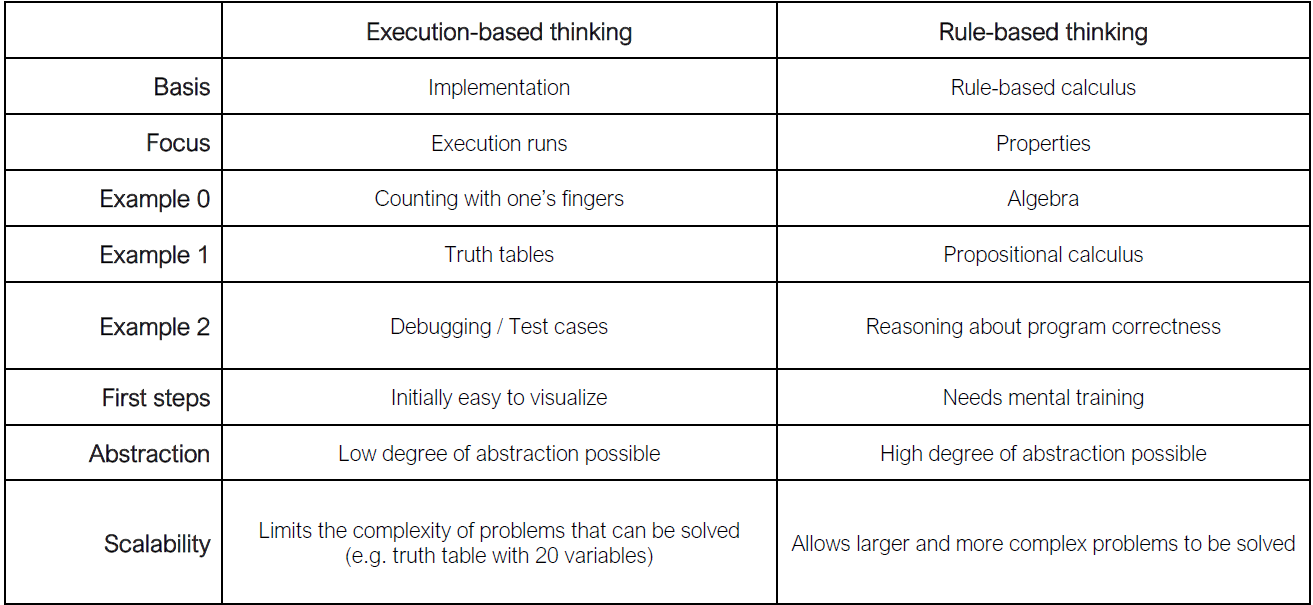
\includegraphics[width=\linewidth]{img/execution_rule_thinking.png}

\section{Programming Paradigms}
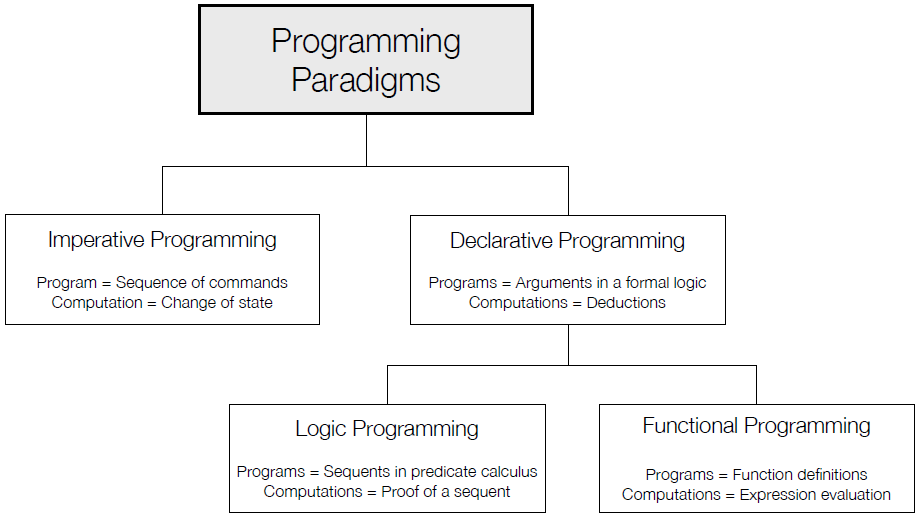
\includegraphics[width=\linewidth]{img/programming_paradigms.png}
\subsection{Imperative}
\begin{itemize}
    \item Befehlend
    \item Focuses on \textbf{how} a program operates
    \item Commands change a program's state
\end{itemize}
\textbf{Common building blocks:}
\begin{itemize}
    \item Assignment: $x := x + 1$
    \item Sequential composition: $(... ; ...)$
    \item Conditional execution: $(if ... then ... else)$
    \item Repetition: $(while ... do ...)$ / $(goto ...)$
\end{itemize}
\subsubsection{Von Neumann architecture}
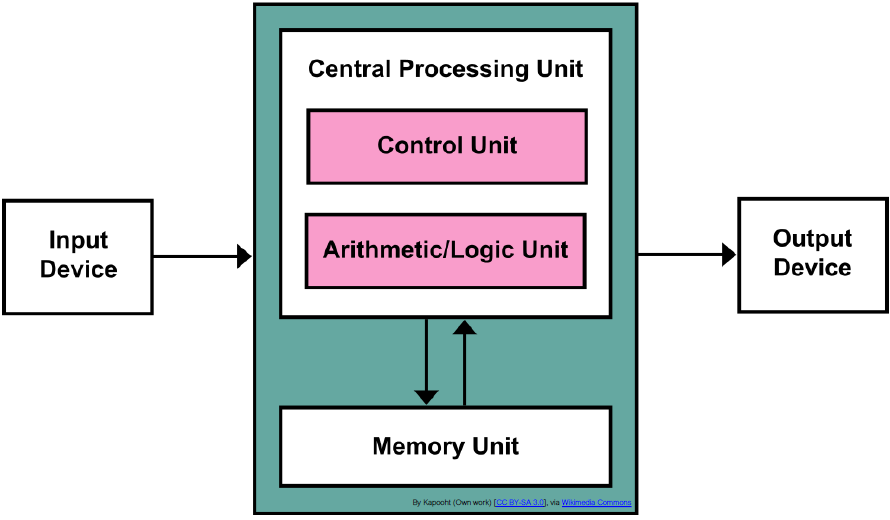
\includegraphics[width=0.7\linewidth]{img/imperative_programming.png}\\

\subsection{Declarative}
\begin{itemize}
    \item Expresses the logic of a computation without describing its control flow
    \item Describes \textbf{what} the program should accomplish
    \item \textbf{how} - left to the language's implementation
    \item eliminates / minimises side effects
\end{itemize}
\textbf{Examples:}
\begin{itemize}
    \item Spreadsheets
    \item Regular expressions
    \item Query languages
    \item Functional programming languages
    \item Logic programming
\end{itemize}

\section{Functional Programming Introduction}
\textbf{Basic Features}
\begin{itemize}
    \item Referential transparency
    \item Functions as first-class citizens
    \item Higher-order functions
    \item Algebraic data types
    \item Pattern matching
    \item Recursion
    \item Types \& type inference
    \item Haskell specific: Type classes, Functors, Applicatives, Monads
\end{itemize}
\textbf{What is FP?}
\begin{itemize}
    \item Declarative programming paradigm
    \item Foundation: Chruch's Lambda calculus
    \item Pure: No (or controlled) mutable state
    \item Pure: Expressions are by default side effect free
\end{itemize}

\textbf{Why functions?}
\begin{itemize}
    \item Simple concept and properties
    \item High level of abstraction possible
    \item Powerful reasoning more easily possible
\end{itemize}

\textbf{Why use FP?}
\begin{itemize}
    \item Easier to reason about
    \item Easier to write
    \item Easier to get right
\end{itemize}

\subsection{No Mutable State}
\begin{itemize}
    \item Referential Transparency: WYSIWYG for programmers
    \item $f(x)$ only depends on the def. of $f$ and the value of $x$
    \item \textbf{No} mutable variables
    \item \textbf{No} assignments
    \item \textbf{No} imperative control structures
    \item All data structures are immutable
\end{itemize}
\textbf{Problem with mutable state}
\begin{itemize}
    \item Every statement can potentially change the underlying state of the program
    \item Executions of a statement can depend on previously executed statements
\end{itemize}

\subsection{Functions are first-class Citizens}
\begin{itemize}
    \item just like any other values: $1, true$
    \item Can be anonymous: $(\lambda x . x + 1)$
    \item Can be input/output to other functions
    \item Can be composed in powerful ways $f o g$
\end{itemize}

\subsection{More FP in the future}
\begin{itemize}
    \item Increased expectations on reliability of software
    \item Increased demands on scalability, complexity, performance
    \item FP can surpass the limitations of the mainstream
    \item FP is an active area of applied research
    \item Increased adoption of FP features in mainstream languages (generics)
\end{itemize}
\columnbreak






        %! Author = Philipp Emmenegger
%! Date = 10/06/2021

\section{Haskell Introduction}
\subsection{Standard Prelude}
\textbf{Select the first element of a list}
\begin{lstlisting}
head [1,2,3,4,5]
1
\end{lstlisting}
\textbf{Remove the first element of a list}
\begin{lstlisting}
tail [1,2,3,4,5]
[2,3,4,5]
\end{lstlisting}
\textbf{Select the nth element of a list}
\begin{lstlisting}
[1,2,3,4,5] !! 2
3
\end{lstlisting}
\textbf{Select the first n elements of a list}
\begin{lstlisting}
take 3 [1,2,3,4,5]
[1,2,3]
\end{lstlisting}
\textbf{Remove the first n elements from a list}
\begin{lstlisting}
drop 3 [1,2,3,4,5]
[4,5]
\end{lstlisting}
\textbf{Calculate the length of a list}
\begin{lstlisting}
length [1,2,3,4,5]
5
\end{lstlisting}
\textbf{Calculate the sum of a list of numbers}
\begin{lstlisting}
sum [1,2,3,4,5]
15
\end{lstlisting}
\textbf{Calculate the product of a list of numbers}
\begin{lstlisting}
product [1,2,3,4,5]
120
\end{lstlisting}
\textbf{Append two lists}
\begin{lstlisting}
[1,2,3] ++ [4,5]
[1,2,3,4,5]
\end{lstlisting}
\textbf{Reverse a list}
\begin{lstlisting}
reverse [1,2,3,4,5]
[5,4,3,2,1]
\end{lstlisting}

\subsection{Function Application Syntax}
\begin{lstlisting}
f a b + c * d
\end{lstlisting}
\begin{itemize}
    \item Function application is denoted using space
    \item Multiplication is denoted using $*$
    \item Function application has higher prio than other operators
\end{itemize}
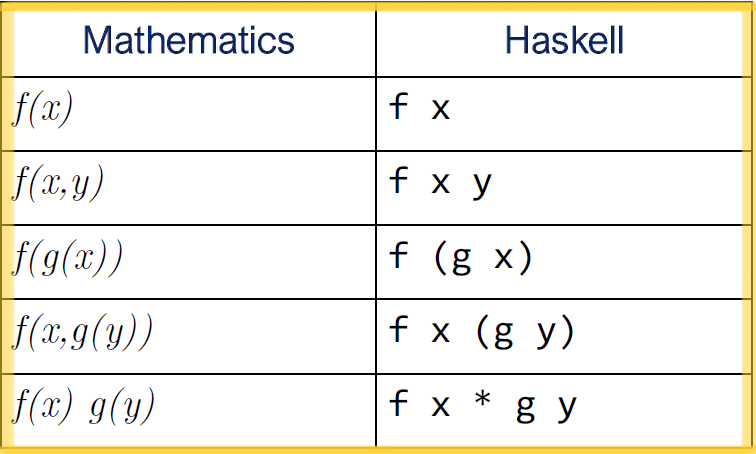
\includegraphics[width=0.6\linewidth]{../img/function_application_syntax.png}\\

\subsection{Useful GHCi Commands}
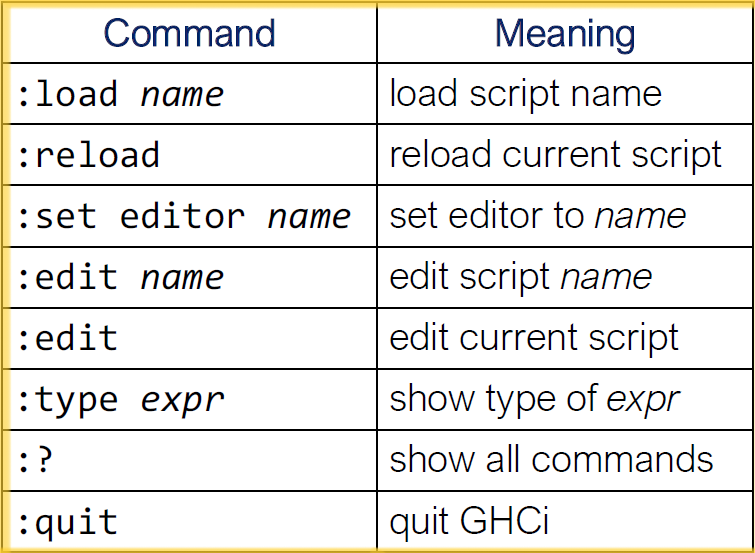
\includegraphics[width=0.6\linewidth]{../img/ghci_commands.png}\\

\subsection{Naming Requirements}
\begin{itemize}
    \item Function and argument names: begin with lowercase letter
    \item List arguments: $s$-suffix, by convention: $xs, ns, nss$
\end{itemize}

\subsection{The Layout Rule}
\begin{itemize}
    \item In a sequence of definitions, definitions must begin in the same column
    \item Avoids the need for braces and semicolons
\end{itemize}














        %! Author = Philipp Emmenegger
%! Date = 10/06/2021

\section{Types and Classes}
\subsection{Type}
\begin{itemize}
    \item Name for a collection of related values
    \item e.g. $Bool = False | True$
    \item Every well-formed expression has a type
    \item Type can be automatically calculated at compile time: \textit{type inference}
    \item Removing the need for type checks at run time => safer /faster
\end{itemize}
\textbf{Type Error}
\begin{itemize}
    \item Applying a function to one or more arguments of the wrong type
\end{itemize}

\subsubsection{Basic Types}
\begin{itemize}
    \item \textbf{Bool}: logical values
    \item \textbf{Char}: single values
    \item \textbf{String}: strings of chars
    \item \textbf{Int}: fixed-precision int
    \item \textbf{Integer}: arbitrary-precision integers
    \item \textbf{Float}: floating-point numbers
\end{itemize}

\subsubsection{List Types}
\begin{itemize}
    \item Sequence of values of the same type
    \item Type of a list says nothing about the length
    \item Lists of lists possible
\end{itemize}
\begin{lstlisting}
[['a'], ['b','c']] :: [[Char]]
\end{lstlisting}

\subsubsection{Tuple Types}
\begin{itemize}
    \item Sequence of values of different types
    \item Type of a tuple encodes its size
    \item Type of components is unrestricted
\end{itemize}
\begin{lstlisting}
(False, 'a', True) :: (Bool, Char, Bool)
\end{lstlisting}

\subsubsection{Function Types}
\begin{itemize}
    \item Mapping from values of one type to values of another
    \item Argument and result types are unrestricted
    \item Functions with multiple arguments / results possible using lists / tuples
\end{itemize}
\begin{lstlisting}
add :: (Int, Int) -> Int
add (x,y) = x + y
\end{lstlisting}

\subsubsection{Curried Functions}
\begin{itemize}
    \item Multiple input arguments typically implemented by returning functions as results
    \item Functions that take their arguments one at a time
    \item Functions with more that two arguments can be curried by returning nested functions
\end{itemize}
\begin{lstlisting}
add' :: Int -> (Int -> Int)
add' x y = x + y
\end{lstlisting}

\subsubsection{Currying Conventions}
\begin{itemize}
    \item $->$ operator is right associative
    \item Rightmost type is the result
    \item Precending types are the input
    \item Consequence: Function application is left associative
    \item All functions in Haskell are normally defined in curried form
\end{itemize}

\subsubsection{Polymorphic Functions}
\begin{itemize}
    \item Function type contains one or more type variables
    \item Type variables must begin with lowercase letters
\end{itemize}
\begin{lstlisting}
length :: [a] -> Int
\end{lstlisting}

\subsubsection{Overloaded Functions}
\begin{itemize}
    \item Function type contains one or more class constraints
    \item Class constraints are expressed as type classes
    \item Can be instantiated to any types that satisfy the constraints
\end{itemize}
\begin{lstlisting}
(+) :: Num a => a -> a -> a
\end{lstlisting}
\textbf{Type classes in Haskell:}
\begin{itemize}
    \item Num: Numeric types
    \item Eq: Equality types
    \item Ord: Ordered types
\end{itemize}
\begin{lstlisting}
(+) :: Num a => a -> a -> a
(==) :: Eq a => a -> a -> Bool
(<) :: Ord a => a -> a -> Bool
\end{lstlisting}

\subsection{Defining Functions}
\subsubsection{Conditional Expressions}
\begin{itemize}
    \item Can be nested
    \item Must always have an else branch
\end{itemize}
\begin{lstlisting}
abs :: Int -> Int
abs n = if n >= 0 then n else -n
\end{lstlisting}

\subsubsection{Guarded Equations}
\begin{itemize}
    \item Make definitions using multiple conditions
    \item Easier to read
\end{itemize}
\begin{lstlisting}
abs n
    | n >= 0 = n
    | otherwise = -n
\end{lstlisting}

\subsubsection{Pattern Matching}
\begin{itemize}
    \item Can be defined many different ways
    \item Some ways may be more efficient
    \item $\_$: wildcard pattern, matches any argument
    \item Patterns are matched in order
    \item Patterns may not repeat variables
\end{itemize}
\begin{lstlisting}
not :: Bool -> Bool
not False = True
not True = False
\end{lstlisting}

\subsubsection{List Patterns}
\begin{itemize}
    \item Non-empty lists are constructed by repeated use of \textit{cons} operator: $(:)$
    \item Functions on lists can be defined using $x : xs$ patterns
\end{itemize}
\begin{lstlisting}
[1,2,3,4] = 1 : (2 : (3 : (4 : [])))
\end{lstlisting}


\subsection{Lambda Expressions}
\begin{itemize}
    \item Used to define anonymous functions
    \item e.g. $\backslash x -> x + x$
    \item Can give a formal meaning to functions defined using currying
\end{itemize}
\begin{lstlisting}
add x y = x + y
add = \x -> (\y -> x + y)
\end{lstlisting}
\textbf{Avoid naming functions that are only referenced once:}
\begin{lstlisting}
odds n = map f [0 .. n - 1]
            where
                f x = x * 2 + 1
odss n = map (\x -> x * 2 + 1) [0 .. n - 1]
\end{lstlisting}

\subsection{Operators}
\begin{itemize}
    \item \textbf{Prefix} notation is used for function application
    \item Is \textbf{Infix} notation desired, one may use operators (e.g. $+$)
    \item Functions can be converted into operators using backticks: $`div`$
    \item Operators can be converted to functions using brackets: $(+)$
\end{itemize}













        %! Author = Philipp Emmenegger
%! Date = 10/06/2021

\section{List Comprehension}
\begin{itemize}
    \item Define functions in very compact manner
    \item Elegant way to perform iteration in declarative style
\end{itemize}
\begin{lstlisting}
factors n = [x | x <- [1 .. n], n `mod` x == 0]
prime n = factors n == [1, n]
primes n = [x | x <- [2 .. n], prime x]
\end{lstlisting}

\subsection{Generators}
\begin{itemize}
    \item States how to generate values for a variable
\end{itemize}
\begin{lstlisting}
x <- [1 .. 5]
\end{lstlisting}
\textbf{Multiple Generators}\\
\begin{itemize}
    \item Order of generators changes order of elements
    \item Multiple generators act like nested loops
\end{itemize}
\begin{lstlisting}
[(x,y) | x <- [1,2,3], y <- [4,5]]
[(1,4),(1,5),(2,4),(2,5),(3,4),(3,5)]
\end{lstlisting}
\textbf{Dependant Generators}
\begin{itemize}
    \item Later generators can depend on variables, introduced by earlier generators
\end{itemize}
\begin{lstlisting}
[(x,y) | x <- [1 .. 3], y <- [x .. 3]]
\end{lstlisting}

\subsection{Guards}
\begin{itemize}
    \item Restrict values produced by earlier generators
\end{itemize}
\begin{lstlisting}
[x | x <- [1 .. 10], even x]
\end{lstlisting}

\subsection{zip - Function}
\begin{itemize}
    \item Maps two lists to a list of pairs
\end{itemize}
\begin{lstlisting}
zip :: [a] -> [b] -> [(a, b)]
\end{lstlisting}

\subsection{String Comprehensions}
\begin{itemize}
    \item String: sequence of chars enclosed in double quotes
    \item Internally strings are represented as lists of chars
    \item Polymorphic list-functions can be applied to strings
\end{itemize}
\begin{lstlisting}
"abc" :: String
['a', 'b', 'c'] :: [Char]
\end{lstlisting}
        %! Author = Philipp Emmenegger
%! Date = 10/06/2021

\section{Recursive Functions}
\subsection{Advantages}
\begin{itemize}
    \item Some functions are simpler to define using recursion
    \item Properties can be proven using induction
\end{itemize}
        %! Author = Philipp Emmenegger
%! Date = 14/07/2021

\section{Higher-Order Functions}
A function is called higher-order if it takes a function as an argument or returns a function as a result.
\begin{lstlisting}
twice :: (a -> a) -> a -> a
twice f x = f (f x)
\end{lstlisting}

\subsection{Why are they useful?}
\begin{itemize}
    \item \textbf{Common programming idioms} can be encoded as functions within the language itself
    \item \textbf{Domain specific languages} can be defined as collections of higher-order functions
    \item \textbf{Algebraic properties} of higher-order functions can be used to reason about programs
\end{itemize}

\subsection{Examples}
\subsubsection{map}
Applies a function to every element of a list.
\begin{lstlisting}
map :: (a -> b) -> [a] -> [b]
-- defined using list comprehension --
map f xs = [f x | x <- xs]
-- defined using recursion --
map f [] = []
map f (x : xs) = f x : map f xs
-- for example: --
map (+1) [1,3,5,7]
[2,4,6,8]
\end{lstlisting}

\subsubsection{filter}
Selects every element from a list that satisfies a predicate.
\begin{lstlisting}
filter :: (a -> Bool) -> [a] -> [a]
-- defined using list comprehension --
filter p xs = [x | x <- xs, p x]
-- defined using recursion --
filter p [] = []
filter p (x : xs)
    | p x = x : filter p xs
    | otherwise = filter p xs
-- example --
filter even [1 .. 10]
[2,4,6,8,10]
\end{lstlisting}

\subsubsection{foldr}
\textbf{Why is foldr Useful?}
\begin{itemize}
    \item Some recursive functions on lists are easier to define
    \item Properties of functions can be proved using albegraic properties of foldr
    \item Advanced program optimisations can be simpler if foldr is used in place of explicit recurison
\end{itemize}
A number of functions on lists can be defined using the following simple pattern of recursion:
\begin{lstlisting}[escapeinside={(*}{*)}]
f [] = v
f (x : xs) = x (*$\bigoplus$*) f xs
\end{lstlisting}
Some function $\bigoplus$ is applied to the head of non-empty lists, and $f$ to its tail.
The value \textbf{v} is typically the identity element of $\bigoplus$.\\
\textbf{For example:}
\begin{lstlisting}
sum [] = 0
sum (x : xs) = x + sum xs

product [] = 1
product (x : xs) = x * product xs

and [] = True
and (x : xs) = x && and xs
\end{lstlisting}
The higher-order library function \textbf{foldr} (fold right) uses this pattern of recursion with the function $\bigoplus$ and the value \textbf{v} as arguments:
\begin{lstlisting}
-- defined using recursion --
foldr :: (a -> b -> b) -> b -> [a] -> b
foldr f v [] = v
foldr f v (x : xs) = f x (foldr f v xs)
-- example --
sum = foldr (+) 0
product = foldr (*) 1
and = foldr (&&) True
-- other examples -- 
length = foldr (\ _ n -> 1 + n) 0
reverse = foldr (\ x xs -> xs ++ [x]) [] 
-- append function (++) --
(++ ys) = foldr (:) ys
\end{lstlisting} 

\subsubsection{Other Library Functions}
\textbf{(.):} returns the composition of two functions as a single function.
\begin{lstlisting}
(.) :: (b -> c) -> (a -> b) -> (a -> c)
f . g = \ x -> f (g x)
-- example --
odd :: Int -> Bool
odd = not . even
\end{lstlisting}
\textbf{all:} decides if every element of a list satisfies a given predicate.
\begin{lstlisting}
all :: (a -> Bool) -> [a] -> Bool
all p xs = and [p x | x <- xs]
-- example --
all even [2,4,6,8,10]
True
adslnasdlasd
\end{lstlisting}
\textbf{any:} decides if at least one element of a list satisfies a predicate.
\begin{lstlisting}
any :: (a -> Bool) -> [a] -> Bool
any p xs = or [p x | x <- xs]
-- example --
any (== ' ') "abc def"
True
\end{lstlisting}
\textbf{takeWhile:} selects elements from a list while a predicate holds.
\begin{lstlisting}
takeWhile :: (a -> Bool) -> [a] -> [a]
takeWhile p [] = []
takeWhile p (x : xs)
    | p x = x : takeWhile p xs
    | otherwise = []
-- example --
takeWhile (/= ' ') "abc def"
"abc"
\end{lstlisting}
\textbf{dropWhile:} drops elements from a list while a predicate holds.
\begin{lstlisting}
dropWhile :: (a -> Bool) -> [a] -> [a]
dropWhile p [] = []
dropWhile p (x : xs)
    | p x = dropWhile p xs
    | otherwise = x : xs
-- example --
dropWhile (== ' ') " abc"
"abc"
\end{lstlisting}
        %! Author = Philipp Emmenegger
%! Date = 10/06/2021

\section{Declaring Types and Classes}
\subsection{Type Declarations}
\begin{itemize}
    \item New name for an existing type
    \item Can make other types easier to read
    \item Can have type parameters
    \item Can be nested
    \item Cannot be recursive
\end{itemize}
\begin{lstlisting}
type String = [Char]
-----------------------
type Pos = (Int, Int)
origin :: Pos
origin = (0, 0)

left :: Pos -> Pos
left (x,y) = (x-1, y)

-- Type parameter --
type Pair a = (a,a)
mult :: Pair Int -> Int
mult (m,n) ) m*n

-- Nested --
type Trans = Pos -> Pos
\end{lstlisting}

\subsection{Data Declarations}
\begin{itemize}
    \item Completely new type by specifying its values
    \item Values of new types can be used the same ways as built in types
    \item Constructors may also have parameters
    \item May also have type parameters
    \item Can be recursive
\end{itemize}
\begin{lstlisting}
data Bool = False | True
data Answer = Yes | No | Unknown

-- Parameter --
data Shape = Circle Float | Rect Float Float
square :: Float -> Shape
square n = Rect n n

-- Type parameters --
data Maybe a = Nothing | Just a

-- Recursive --
data Nat = Zero | Succ Nat
Succ (Succ (Succ Zero)) = 3
\end{lstlisting}

\subsection{Polymorphism}
\begin{enumerate}
    \item Ad-hoc Polymorphism: function with the same name denotes different implementations (function overloading / interfaces)
    \item Parametric Polymorphism: Code written to work with many possible types
    \item Subtype Polymorphism: one type can be substituted for another (subtype / supertype)
\end{enumerate}

\subsection{Type Classes}
\begin{itemize}
    \item Declared using class declarations
\end{itemize}
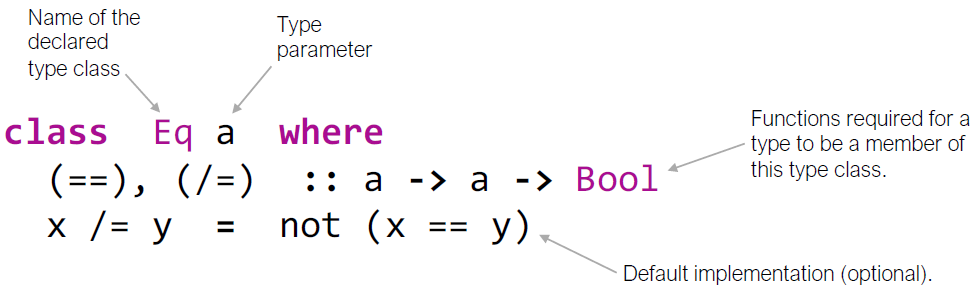
\includegraphics[width=0.7\linewidth]{img/class_declarations.png}
        %! Author = Philipp Emmenegger
%! Date = 14/07/2021

\section{Lambda Calculus}
\begin{itemize}
    \item Indroduced by Alonzo Church in 1930s
    \item Part of an investigation into the foundations of mathematics
    \item Expresses computation based on function abstraction
    \item Expresses application using variable binding and substitution
    \item Most compact and elegant programming language
    \item Basics for functional programming
    \item \textbf{Pure:} no pre-defined constants
    \begin{itemize}
        \item Only reserved words: '$\lambda$', '.', '(' and ')',
    \end{itemize}
    \item Proofs that function evaluation is enough for functional programming
\end{itemize}

\subsection{Sequents in LC}
Sequents in \textbf{LC} have the identical form as in\\
\textbf{PC} (Propositional Calculus) and \\ 
\textbf{FoPCe} (First-Order Predicate Calculus with Equality).\\
\begin{center}
    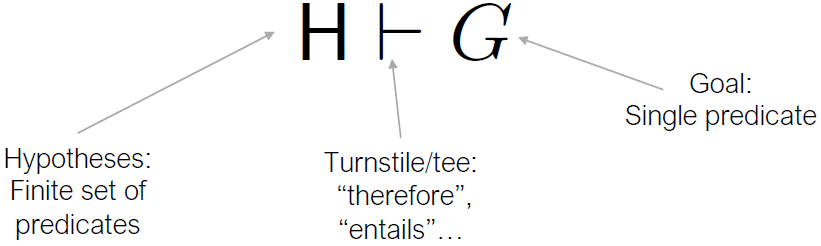
\includegraphics[width=0.8\linewidth]{img/sequents_lc.png}\\
    \textbf{\textit{Under the hypotheses H, prove the goal G}}
\end{center}

\subsection{Syntax in LC}
Formulae in LC can eiter be:
\begin{itemize}
    \item predicates (P)
    \item $\lambda$-Terms (M)
\end{itemize}
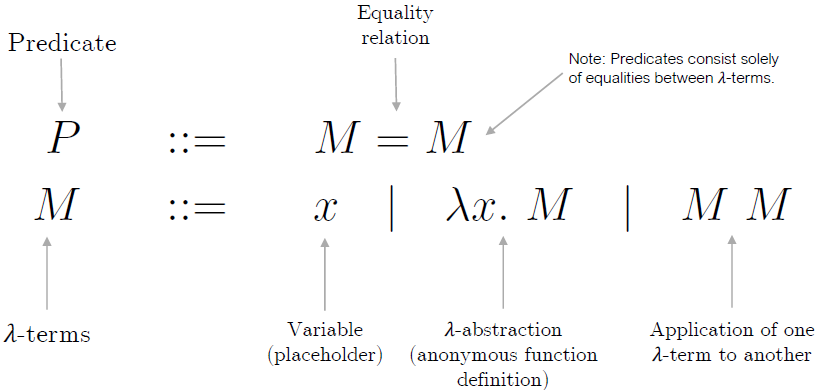
\includegraphics[width=\linewidth]{img/lc_syntax.png}

\subsubsection{Conventions}
\textbf{Application binds tighter than abstraction}\\
$\lambda x.M_1 M_2$ represents $\lambda x.(M_1M_2)$ and not $(\lambda x.M_1) M_2$\\ 
\textbf{Application is left associative}\\ 
$M_1 M_2 M_3$ represents $(M_1 M_2) M_3$ and not $M_1 (M_2 M_3)$

\subsubsection{Free and Bound Variables}
Bound variables are basically placeholders. 
Their names have no significance and can be renamed.\\
\begin{center}
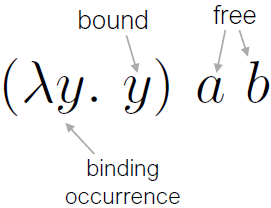
\includegraphics[width=0.2\linewidth]{img/lc_variables.png}
\end{center}
\textbf{$\alpha$-equivalence:}\\
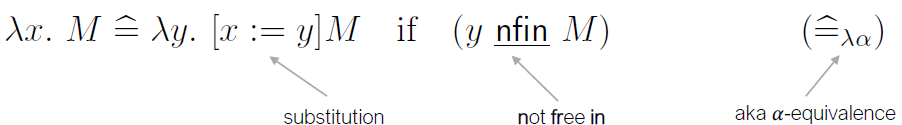
\includegraphics[width=\linewidth]{img/lc_alpha.png}

\subsubsection{Proof rules of LC}
Lambda Calculus contains only one proof rule schema of major significance: \textbf{$\beta$-reduction}\\ 
\begin{center}
    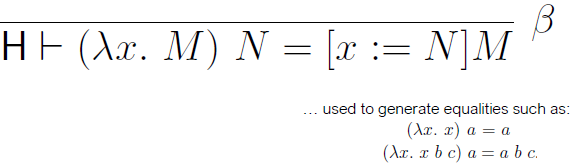
\includegraphics[width=0.8\linewidth]{img/lc_beta.png}
\end{center}
$\beta$-Reduction defines what function application means in the context of lambda calculus. 
It states that applying a lambda abstraction $(\lambda x.M)$ to another lambda term $(N)$ results in all occurences of the formal parameter $(x)$ within the body of the abstraction $(M)$ being replaced with the actual parameter $(N)$ supplied.\\\\ 
\begin{center}
    $\frac{(\lambda x. \; square \; x)\; 5}{=\; square \; 5}$\\
    \vspace{0.5cm}
    $\frac{(\lambda x. \; square \; x) \: (\lambda y. \; square \; y) \; 5}{= \; (square \; (\lambda y. \; square \; y)) \; 5}$
\end{center}

\subsection{Computation with LC}
Computation in the lambda calculus is done by repeatedly applying the rule schema $\beta$ to achieve $\beta$-reduction.\\ 
\begin{center}
    \textbf{Evaluation in LC = Reduction}
\end{center}

\subsubsection{Normal Form}
A $\lambda$-term is said to be in \textbf{normal form} if no further reductions can be applied to it.
It is possible for a $\lambda$-term to offer several opportunities for reduction simultaneously:
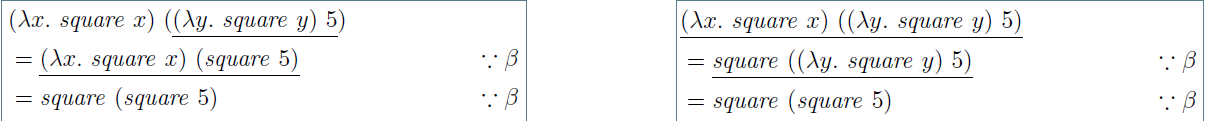
\includegraphics[width=\linewidth]{img/lc_reduction.png}
\textbf{Confluence:} Every $\lambda$-term has at most one normal form

\subsubsection{Function Application Syntax}
Functions are \textbf{first-class citizens}. Functions and their arguments belong to the same syntactic category.
\begin{itemize}
    \item Prefix notation is used instead of infix notation
    \item Parameters do not need to be enclosed in parantheses
\end{itemize}

\subsubsection{Currying}
\textbf{Motivation:} LC only allows unary (1 argument) function application.\\ 
\textbf{Currying:} A function with several arguments can be thought of as a series of higher order functions, each with being unary.
\begin{itemize}
    \item Not just a smart syntactic trick
    \item Makes functional definitions more concise, modular and reusable
\end{itemize}

\subsubsection{Definitions}
\begin{itemize}
    \item Not strictly necessary 
    \item Sometimes convenient
    \item Adding definitions as equalities within the hypotheses of LC sequents
\end{itemize}
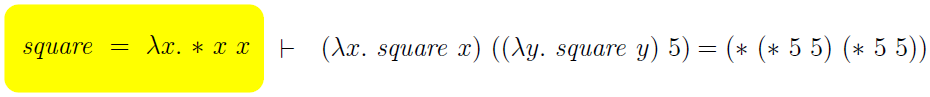
\includegraphics[width=\linewidth]{img/lc_definitions.png}

\subsubsection{Delta-Reduction}
\textbf{$\delta$-Reduction:} substitution of a defined symbol with its definition\\
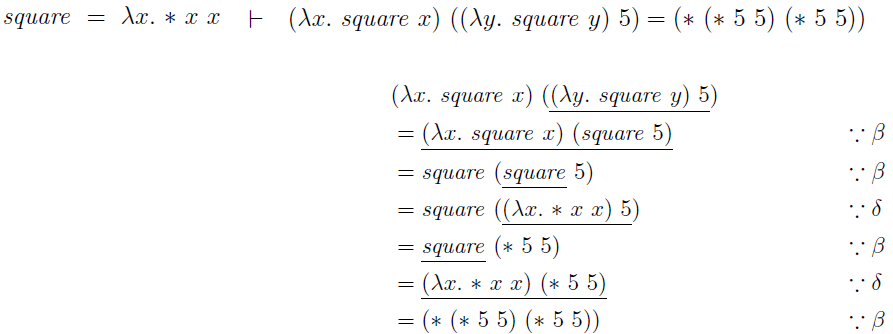
\includegraphics[width=\linewidth]{img/lc_delta.png}

\subsection{Evaluation Strategies}
\textbf{redex:} reducible expression (any $\beta \delta$-reducible sub-term)\\ 
\textbf{evaluation strategy:} order in which redexes are reduced
\begin{itemize}
    \item $\lambda$-terms may have more than one redex at any stage of the evaluation
    \item LC does not place any constraints on the order in which redexes are reduced
    \item The order plays an important role in the \textbf{length of derivations} and their \textbf{termination}
\end{itemize}

\subsubsection{Leftmost Innermost (aka. applicative order / innermost first)}
\begin{enumerate}
    \item The innermost redex is reduced First
    \item In case there is more than one innermost redex, the leftmost innermost redex is reduced First
\end{enumerate}
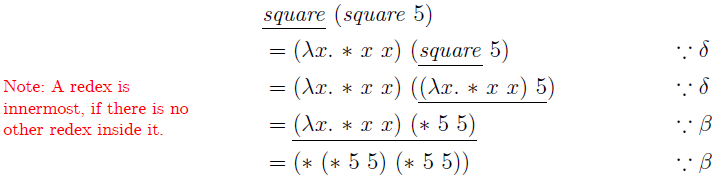
\includegraphics[width=0.9\linewidth]{img/lc_innermost.png}
\begin{itemize}
    \item A functions arguments are substituted into the body of a function after they are reduced
    \item A functions arguments are reduced exactly once
    \item Parameter passing: \textbf{Call by value}
\end{itemize}

\subsubsection{Leftmost Outermost (aka. normal order / outermost first)}
\begin{enumerate}
    \item The outermost redex is reduced First
    \item In case there is more than one outermost redex, the leftmost-outermost redex is reduced First
\end{enumerate}
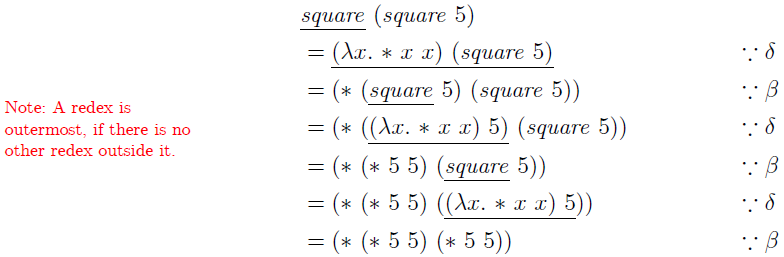
\includegraphics[width=0.9\linewidth]{img/lc_outermost.png}
\begin{itemize}
    \item A functions arguments are substituted into the body of a function before they are reduced
    \item A functions arguments are reduced as often as they are needed
    \item \textbf{If a normal form exists, leftmost outermost will find it}
    \item Parameter passing: \textbf{Call by name}
\end{itemize}

\subsubsection{Lazy Evaluation}
Implementation technique to make call by name more efficient.
Uses memorizing (caching) to avoid computing the same expression more than once.
\textbf{Default for Haskell}

\subsection{Encoding Data and Operations}
The pure lambda calculus \textbf{does not have any primitive data types} such as Booleans, numbers, tuples, etc.\\ 
\subsubsection{Boolean Algebra}
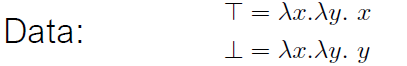
\includegraphics[width=0.5\linewidth]{img/lc_data.png}
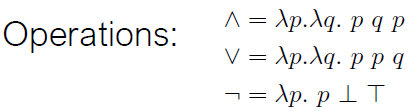
\includegraphics[width=0.5\linewidth]{img/lc_operations.png}
\subsubsection{Arithmetic}
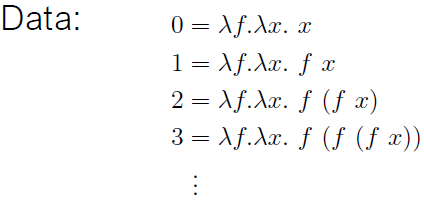
\includegraphics[width=0.35\linewidth]{img/lc_data2.png}
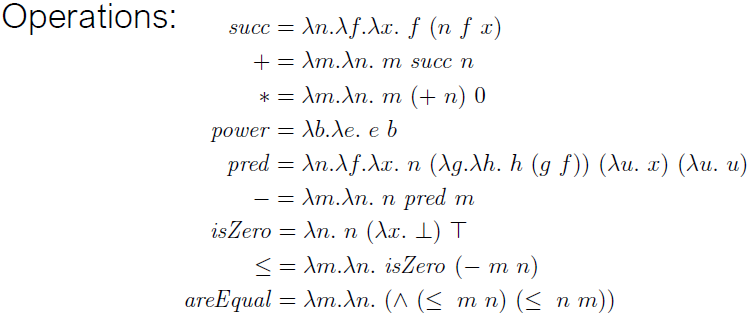
\includegraphics[width=0.65\linewidth]{img/lc_operations2.png}
\subsubsection{Pairs}
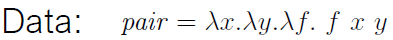
\includegraphics[width=0.5\linewidth]{img/lc_data3.png}
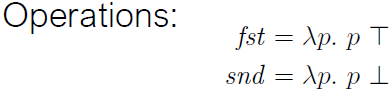
\includegraphics[width=0.5\linewidth]{img/lc_operations3.png}

    \end{multicols*}
\end{document}

























